\ofsubsection{Profissões}
%
%
%
\ofjob{Bardo}
{
	\ofquote{"Bem vindo ao seu fim, estrelando: euzinha!"\\}{Rikku}\\\\
	
\includegraphics[width=\columnwidth]{./art/jobs/bard.jpg}\ofrow
	\accf{Bardos} estão na fronteira entre a arte e a guerra.
	Eles podem realizar canções e danças que concedem poderosos benefícios à aliados e dificuldades terríveis aos inimigos.
	Entretanto, Bardos não são os duelistas mais poderosos, em geral eles viram a maré da batalha de maneiras inesperadas.
}
{Adaga}{Armadura Leve ou Robe}{
	Nível 1: & PV~+19 & PM~+20 & AGI~+3 & RES~+1  \\
	Nível 2: & PV~+10  & PM~+10 & DEF~+1  \\
	Nível 3: & \multicolumn{3}{l}{Bônus de Atributo do Arquétipo} \\
	Nível 4: & PV~+5  & PM~+10 & RES~+1 & DEF~+1 \\
	Nível 5: & PV~+10 & PM~+5  & FOR~+2 \\ 
	Nível 6: & PV~+5  & PM~+10 & RES~+1 & DEF~+1 \\
	Nível 7: & PV~+10 & PM~+10 & FOR~+1 &  	  \\
	Nível 8: & PV~+10  & PM~+10 & DEF~+1 \\
	Nível 9: & PV~+10 & PM~+10 & FOR~+1 \\
	Nível 10: & PV~+5  & PM~+10 & RES~+1 & DEF~+1	
}{
	\ofjobtech{Torcida}{4}{0r}{1u}{Você}{Todos na área podem escolher um dos seguintes benefícios: \mbox{AuFOR}, AuMAG, AuDEF or AuRES por 3 rodadas.}{\enstr\enmag}{1}\ofabilitygap
	\ofjobtech{Improvisação}{6}{0r}{Único}{5u}{Role 1d. Baseado no resultado, o alvo recebe o seguinte Efeito de Estado por 3 rodadas: 1-AuDEF, 2-AuRES, 3-AuSTR, 4-Oscilando, 5-Regenerando, 6-Acelerado.}{\enndef\enres\enstr\blink\regen\haste}{2}\ofabilitygap
	\ofjobtech{Sob os holofotes}{8}{0r}{2u}{Você}{Crie um campo Obscuro ao seu redor, que o segue por 3 rodadas, mas não o afeta.}{}{4}\ofabilitygap
	\ofjobtech{Marcha poderosa}{14}{0r}{2u}{Você}{Você e seus aliados na área de efeito recebem Acelerado e AuDEF por 2 rodadas.}{\haste\enndef}{6}\ofabilitygap
	\ofjobtech{Encantar}{15}{1r}{Único}{4u}{Escolha um inimigo como alvo. Ele faz um teste de DF~8 ou imediatamente tem mais um turno para agir sob seu comando. Alguns inimigos são Imunes a esse efeito.}{}{8}\ofabilitygap
	\ofjobtech{Imitar}{?}{0r}{?}{?}{Copie uma habilidade usada por um aliado ou inimigo no campo de batalha desde o turno anterior. Ao fazer isso, esteja sujeito ao custo de PM, tempo de conjuração, assim como, alcance e alvo da habilidade copiada.}{}{10}
}{
	\ofarchetypet{Dançarino(a)}
	{PV~+12 & PM~+8 & FOR~+2 & DEF~+1}
	{\ofarchetypetecha{Dança das lâminas}{6}{0r}{Único}{1u}{Ataque o alvo. Então escolha outro alvo dentro de 2u, corra em sua direção e o ataque também.}{}}
	{\ofspecial{Vestido(a) para matar}{Equipe um acessório extra. Além disso, para cada acessório equipado, você pode escolher um benefício extra entre: DEF+1 ou RES+1.}{5}{\oficonpassive}}	
	{\ofspecial{Dança indecente}{Sempre que se evadir de um ataque com sucesso, inflija um dos seguintes Efeitos de Estado ao atacante, por 3 turnos: Imóvel, Envenenado, Cego.}{7}{\oficonreaction}}
	{\ofarchetypetechb{Dança Lenta}{12}{0r}{2u}{Você}{Crie um campo especial ao seu redor que dura por 3 rodadas, agindo como um campo Ardente e Vagaroso. O campo se move com você e afeta somente inimigos.}{}}
}{
	\ofarchetypet{Cantor(a)}
	{PV~+4 & PM~+16 & RES~+3}
	{\ofarchetypetecha{Réquiem}{8}{0r}{Único}{4u}{O alvo faz um teste de DF~8 ou sofre dano de escuridão igual a 2x seu Nível atual e a condição Zumbi por 3 rodadas.}{\zombie\dark}}
	{\ofarchetypepassive{Bis}{Sempre que conceder um ou mais Efeitos de Estado positivos a um alvo, também restaure o PV dele igual ao seu Nível atual.}}
	{\ofarchetypereaction{Dueto}{Sempre que um aliado dentro de 1u realiza um ataque ou usa uma habilidade no inimigo, imediatamente use a mesma habilidade em um aliado ou alvo afetado, se ele estiver ao alcance.}}
	{\ofarchetypetechb{Canção de ninar}{12}{0r}{2u}{5u}{Inimigos na área de efeito fazem um teste de DF~8 ou sofrem 3d de dano e estão Adormecidos por 3 rodadas.}{\sleep}}
}
%
%
%
\ofjob{Mago Negro}
{
	\ofquote{"De fato, você é um ótimo observador do óbvio, kupo!"\\}{Montblanc}\\\\
	
\includegraphics[width=\columnwidth]{./art/jobs/blackmage2.jpg}\ofrow
	\accf{Magos Negros} são frágeis em combates físicos, mas podem acabar com os inimigos à distância com magias poderosas.
	Garantem grande controle sobre o campo de batalha e são difíceis de serem ignorados pelos inimigos.
}
{Cajado}{Robe}{
	Nível 1: & PV~+18 & PM~+26 & AGI~+2 & RES~+1  \\
	Nível 2: & PV~+5  & PM~+10 & MAG~+1 & FOR~+1  \\
	Nível 3: & \multicolumn{3}{l}{Bônus de Atributo do Arquétipo} \\
	Nível 4: & PM~+10 & RES~+1 & DEF~+1 & MAG~+1 	\\
	Nível 5: & PV~+10 & PM~+10 & MAG~+1 		  \\
	Nível 6: & PV~+5  & PM~+10 & RES~+1 & MAG~+1 \\
	Nível 7: & PV~+5  & PM~+10 & MAG~+1 & RES~+1 \\
	Nível 8: & PV~+5  & PM~+10 & RES~+1 & DEF~+1 \\
	Nível 9: & PV~+5  & PM~+10 & RES~+1 & MAG~+1  \\
	Nível 10: & PV~+10 & PM~+10 & MAG~+1		  
}{
	\ofjobspell{Fogo}{4}{0r}{Único}{3u}{Cause 2d de dano de Fogo ao alvo.}{\fire}{1}\ofabilitygap
	\ofjobspell{Nevasca}{4}{0r}{Único}{3u}{Cause 2d de dano de Gelo ao alvo.}{\ice}{1}\ofabilitygap
	\ofjobspell{Raio}{4}{0r}{Único}{3u}{Cause 2d de dano de Raio ao alvo.}{\lightning}{1}\ofabilitygap
	\ofjobspell{Cego}{6}{0r}{Único}{5u}{O alvo faz um teste de DF~8 ou fica Cego por 3 rodadas.}{\blind}{2}\ofabilitygap
	\ofjobspell{Fogaga}{12}{1r}{Único}{5u}{Cause 6d de dano de Fogo ao alvo.}{\fire}{6}\ofabilitygap
	\ofjobspell{Nevasga}{12}{1r}{Único}{5u}{Cause 6d de dano de Gelo ao alvo.}{\ice}{6}\ofabilitygap
	\ofjobspell{Raiaga}{12}{1r}{Único}{5u}{Cause 6d de dano de Raio ao alvo.}{\lightning}{6}\ofabilitygap
	\ofjobspell{Labareda}{25}{2r}{Único}{7u}{Cause 6d+45 de dano ao alvo, ignorando a RES dele.}{\fire}{8}\ofabilitygap
	\ofjobspell{Última}{30}{2r}{50u}{Você}{Cause 6d+40 de dano de escuridão a todos os inimigos na área de efeito.}{\dark}{10}
}{
	\ofarchetypet{Geomante}
	{PV~+14 & PM~+6 & DEF~+2 & RES~+1}
	{\ofarchetypespella{Bio}{8}{0r}{Único}{5u}{O alvo faz um teste de DF~8 ou sofre 3d de dano de Envenenado por 3 turnos.}{\poison}}
	{\ofarchetypepassive{Campo elemental}{Ao conjurar uma magia que cause dano de Fogo, Gelo ou Raio, também crie um campo ao redor do alvo de área até 2u, que dura por 1 rodada. O efeito do campo depende do elemento da magia: Fogo - Campo Ardente, Gelo - Campo Derrapante ou Raio - Campo Vagaroso.}}
	{\ofarchetypereaction{Escudo de Gaia}{Ao sofrer dano elemental, dobre sua DEF ou RES para calcular o dano recebido.}}
	{\ofarchetypespellb{Terremoto}{18}{1r}{3u}{10u}{Cause 6d+5 de dano de terra a todos na área de efeito.}{\earth}}
}{
	\ofarchetypet{Acadêmico}
	{PV~+7 & PM~+18 & MAG~+2}
	{\ofarchetypespella{Tese}{8}{0r}{Único}{5u}{Escolha um tipo de ação, por exemplo Ataque ou Magia. Se o alvo realizar tal ação no próximo turno dele, ele sofre dano igual ao nível dele x2 e fica Imóvel por 2 rodadas.}{}}
	{\ofarchetypepassive{Análise}{Ao causar danos mágicos, aprenda um dos seguintes aspectos sobre o alvo: Resistências, Fraquezas, Imunidades, PV ou PM atuais.}}
	{\ofarchetypereaction{Aprender}{Ao ser alvo de Magias, faça um teste de DF~8. Em caso de sucesso, aprenda como usar a mesma magia. Caso já tenha aprendido alguma magia dessa forma, é possível substituir pela nova.}}
	{\ofarchetypespellb{Especializar}{5}{0r}{Único}{5u}{Escolha uma habilidade do alvo. Pelas próximas 3 rodadas, quando ele usar essa habilidade, seu alcance é dobrado e seu custo em PM, reduzido pela metade.}{\ko}}
}
%
%
%
\ofjob{Dragoon}
{
	\ofquote{"Desgraçado cheio de si, não é?"\\}{Kain}\\\\
	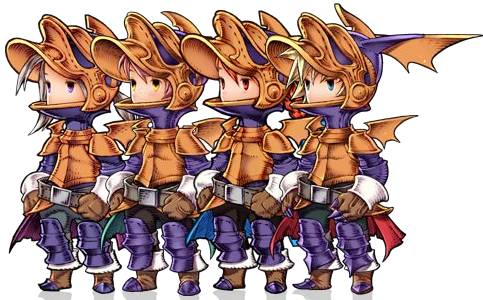
\includegraphics[width=\columnwidth]{./art/jobs/dragoon.jpg}\ofrow
	\accf{Dragoon} são mestres do combate aéreo, atacando seus inimigos com golpes devastantes vindos do céu.
	Preferem empunhar lanças e têm afinidade ao elemento Fogo.
	Mesmo sendo humanoides, é dito que possuem a alma de um dragão. 
}
{Lança}{Armadura Pesada}{
	Nível 1: & PV +23 & PM~+16 & AGI~+2,& FOR~+1 \\
	Nível 2: & PV~+10  & PM~+5 & FOR~+1 & RES~+1 \\
	Nível 3: & \multicolumn{3}{l}{Bônus de Atributo do Arquétipo} \\
	Nível 4: & PV~+5  & PM~+10 & DEF~+2 &  	  \\
	Nível 5: & PV~+10 & PM~+10 & FOR~+1 & 		  \\ 
	Nível 6: & PV~+10 & PM~+10 & RES~+1 		  \\
	Nível 7: & PV~+10 & PM~+5  & FOR~+1 & 	DEF~+1	  \\ 
	Nível 8: & PV~+10 & PM~+10 & RES~+1 & 	 	  \\ 
	Nível 9: & PV~+10  & PM~+10 & FOR~+1 \\ 
	Nível 10:& PV~+10  & RES~+1 & DEF~+2 
}{
	\ofjobtech{Salto}{4}{1r}{Único}{3u}{Ao começar a usar essa técnica, salte até 3u no ar. Após a conjuração, salte sobre o alvo e o ataque.}{}{1}\ofabilitygap
	\ofjobtech{Lanceta}{3}{0r}{Único}{5u}{Cause dano ao PV e PM do alvo igual ao seu nível atual e aumente seu próprio PV e PM na mesma quantidade. Este valor não é reduzido pela DEF ou RES do alvo.}{}{2}\ofabilitygap
	\ofjobtech{Salto duplo}{8}{1r}{Único}{3u}{Ao começar a usar essa técnica, salte até 3u no ar. Após a conjuração, salte sobre o alvo e o ataque. É possível saltar até outro local dentro de 3u. Se aterrizar em outro inimigo, ataque-o ao invés.}{}{6}\ofabilitygap
	\ofjobtech{Rugido}{8}{0r}{5u}{Você}{Inimigos na área de efeito fazem um teste de DF~9 ou sofrem 2d de dano e ficam Imóveis por 1 rodada. }{\immobile}{8}\ofabilitygap
	\ofjobtech{Ventania}{24}{1r}{Único}{Você}{Por 3 rodadas, você permanece até 3u no ar, de onde você pode ser mover normalmente e realiza uma das seguintes ações, sem custo de PM adicional:\\ 
		\acc{Rajada de Lança:} ataque o alvo uma vez, dentro de 10u. Em caso de sucesso, considere um Acerto Crítico.\\
		\acc{Explosão de Fogo:} escolha um alvo dentro de 10u. Ele e inimigos dentro de 2u dele sofrem 4d de dano de Fogo.}{\fire}{10}
}{
	\ofarchetypet{Cavaleiro do Dragão}
	{PV~+8 & PM~+12 & FOR~+1 & RES~+2}
	{\ofarchetypetecha{Baforada de Fogo}{7}{0r}{3u (Frontal)}{Você}{Cause 2d de dano de Fogo a todos na área de efeito.}{\fire}}
	{\ofarchetypepassive{Flamígera}{Ganhe Resistência permanente contra Fogo. Além disso, sempre que causar danos físicos, você pode escolher fazer com que o dano seja inteiramente mágico e do tipo fogo.}}
	{\ofarchetypereaction{Coração de Dragão}{Sempre que causar ou receber dano de Fogo, ganhe AuFOR até o fim de seu próximo turno.}}
	{\ofarchetypetechb{Mergulho do Dragão}{16}{1r}{3u}{7u}{Ao começar a usar essa técnica, salte até 3u no ar. Após a conjuração, salte sobre o alvo e cause 4d de dano de Fogo, além disso, crie um campo Ardente na área do alvo, que dura por 3 rodadas, mas não afeta a você.}{\fire}}
}{
	\ofarchetypet{Valquíria}
	{PV~+13 & PM~+7 & FOR~+2 & DEF~+1}
	{\ofarchetypetecha{Grande Impulso}{6}{0r}{5u (Linha)}{Você}{Corra em frente até 5u em linha. Ataque todos no caminho rolando danos uma vez para cada alvo que falhe em se evadir.}{}}
	{\ofarchetypepassive{Duelista}{Enquanto estiver em combate dentro de 3u de um inimigo e não haja outra pessoa dentro de 3u de você, o bônus de FOR para seus ataques e habilidades é dobrado.}}
	{\ofarchetypereaction{Ao alcance da mão}{Sempre que um inimigo passa a 2u de você, ele faz um teste de DF~7 ou não pode se mover além de você nesse turno.}}
	{\ofarchetypetechb{Vingança}{16}{0r}{Único}{1u}{Ataque um inimigo que  tenha causado danos a você desde o turno anterior. Se acertar, cause o dano que ele te causou antes de causar o seu próprio.}{}}
}
%
%
%
%
%
\ofjob{Atirador}
{
	\ofquote{"Eu sou o protagonista; Quem mais?"\\}{Balthier}\\\\
	
\includegraphics[width=\columnwidth]{./art/jobs/marksman.jpg}\ofrow
	\accf{Atirador} são peritos com todos os tipos de armas à distância.
	Atiradores habilidosos podem ver através de seus inimigos, o que os permite saber as forças e fraquezas deles. 
	Portanto, podem não somente causar danos significativos à distância, mas também, incapacitá-los com técnicas especiais.
}
{Arco ou Arma de fogo}{Armadura Leve}{
	Nível 1: & PV +19 & PM~+17 & AGI~+2 & FOR +1 \\
	Nível 2: & PV~+10  & PM~+10 & DEF~+1 \\
	Nível 3: & \multicolumn{3}{l}{Bônus de Atributo do Arquétipo}  \\
	Nível 4: & PV~+5  & PM~+5  & FOR~+2 & RES~+1 \\
	Nível 5: & PV~+5  & PM~+10 & DEF~+1 & RES~+1  \\
	Nível 6: & PV~+10 & PM~+10 & RES~+1 &        \\
	Nível 7: & PV~+5  & PM~+10 & FOR~+1 & RES~+1 \\
	Nível 8: & PV~+10  & PM~+5 & DEF~+2 		  \\
	Nível 9: & PV~+5  & PM~+10 & RES~+1 & FOR~+1 \\
	Nível 10:& PV~+10 & PM~+10 & FOR~+1 &        
}{
	\ofjobtech{Libra}{4}{0r}{Único}{5u}{Analise o alvo completamente e saiba suas Resistências, Fraquezas, Imunidades e seus PV e PM atuais.}{}{1}\ofabilitygap
	\ofjobtech{Disparo Pesado}{6}{0r}{Único}{Arma}{Ao atacar com sucesso, seu dano ignora a DEF.}{}{2}\ofabilitygap
	\ofjobtech{Saque Rápido}{8}{0r}{Único}{Arma}{Ataque e logo após você pode usar uma habilidade no mesmo turno.}{}{4}\ofabilitygap
	\ofjobtech{Disparo Explosivo}{10}{0r}{2u}{arma}{Alvos na área de efeito sofrem 3d de dano de Fogo. Além disso, crie um Campo Ardente na área do alvo, que dura por 3 rodadas.}{\fire}{6}\ofabilitygap
	\ofjobtech{Bomba de Fumaça}{10}{0r}{3u}{10u}{Crie um Campo Obscuro na área do alvo, que dura por 3 rodadas.}{}{8}\ofabilitygap
	\ofjobtech{Rajada}{24}{1r}{Único}{Você}{Receba Acelerado e AuFOR por 3 rodadas. Além disso, seus ataques que atinjam um único alvo, acertam todos os inimigos dentro de 2u do alvo escolhido.
	}{\haste\enstr}{10}
}{
	\ofarchetypet{Patrulheiro}
	{PV~+13 & PM~+12 & DEF~+2}
	{\ofarchetypetecha{Armar Armadilha}{5}{0r}{1u}{Você}{Arme uma armadilha onde está. Um inimigo que passar sobre ela sofre dano igual ao seu nível atual e fica Imóvel por 1 rodada. A armadilha desaparece após ser ativada.}{\immobile}}
	{\ofarchetypepassive{Recuo}{Ao atacar com sucesso, você pode se mover 1u em qualquer direção de imediato.}}
	{\ofarchetypereaction{Evasão Mágica}{Se evada de Magias ao passar no teste de evasão. Ao fazer isso num Ataque ou Magia, recupere PM igual ao seu Nível.}}
	{\ofarchetypetechb{Munição Envenenada}{10}{0r}{Único}{Arma}{Ao atacar com sucesso, o dano causado é mágico e o alvo faz um teste de DF~8 ou fica Envenenado e recebe ReFOR e ReDEF por 3 rodadas.}{\poison\destr\dedef}}
}{
	\ofarchetypet{Atirador de Elite}
	{PV~+5 & PM~+15 & FOR~+3}
	{\ofarchetypetecha{Disparo Perfurante}{6}{0r}{10u (Linha)}{Você}{Ataque todos em uma linha, role um dano que servirá para todos que falharem no teste de evasão.}{}}
	{\ofarchetypepassive{Concentrado}{Ao atacar um inimigo, ele terá Desvantagem no teste de evasão.}}
	{\ofarchetypereaction{Camuflagem}{Ao fim de seu turno, no qual não tenha se movido, você fica Oscilando até o início de seu próximo turno.}}
	{\ofarchetypetechb{Mirar}{8}{0r}{Único}{Arma}{Ataque o alvo e escolha uma das seguintes partes para efeito adicional:\\ \acc{Cabeça:} a DF de evasão do alvo é reduzida em 2, somente se você obter um Acerto Crítico.\\ \acc{Coração:} O PM do alvo é reduzido pelo mesmo valor de PV.\\ \acc{Perna:} O alvo fica Imóvel por 1 rodada.}{\immobile}}
}
%
%
%
%
%
\ofjob{Monge}
{
	\ofquote{"Agora sei o porquê de seus músculos estúpidos!"\\}{Sabin}\\\\
	
\includegraphics[width=\columnwidth]{./art/jobs/monk2.jpg}\ofrow
	\accf{Monges} São lutadores adeptos ao combate físico que possuem uma combinação mortal de força e técnica.
	Embora não tenha perícia no uso de magias, podem produzir efeitos parecidos a partir de sua força interior.
}
{Nenhuma}{Armadura Leve}{
	Nível 1: & PV +20 & PM~+16 & AGI~+4 & \\
	Nível 2: & PV~+10 & PM~+5  & FOR~+2 & \\
	Nível 3: & \multicolumn{3}{l}{Bônus de Atributo do Arquétipo} \\
	Nível 4: & PV~+5  & PM~+10 & FOR~+1 & RES~+1 \\
	Nível 5: & PV~+10  & PM~+5 & DEF~+1 & FOR~+1 \\
	Nível 6: & PV~+10 & PM~+5  & FOR~+1 & RES~+1 \\
	Nível 7: & PV~+10 & PM~+5  & FOR~+1 & DEF~+1 \\ 
	Nível 8: & PV~+10 & PM~+5  & DEF~+2 &        \\
	Nível 9: & PV~+5  & PM~+10 & FOR~+1 & RES~+1 \\ 
	Nível 10: & PV~+10 & PM~+10 & DEF~+1 &        \\ 
}{
	\ofjobpassive{Combatente Desarmado}{Em combate, use seus punhos como armas. Eles têm o mesmo dano de armas da maior categoria que você usa. Além disso, você pode carregar um terceiro acessório no lugar de seu espaço para armas e receber FOR +1 para cada um deles equipados. Você também pode por uma Matéria no acessório que utiliza no lugar de uma arma.}{1}\ofabilitygap
	\ofjobtech{Chute}{4}{0r}{1u}{Você}{Ataque todos os inimigos dentro de 1u ao seu redor, rolando um dano para todos que falharem no teste de evasão, os quais também serão afastados 1u de você.}{}{2}\ofabilitygap
	\ofjobtech{Aura Explosiva}{6}{0r}{Único}{3u}{Cause dano mágico ao alvo igual ao seu nível atual.}{}{4}\ofabilitygap
	\ofjobtech{Esmurrar}{8}{0r}{Único}{1u}{Ataque o mesmo alvo 2 vezes.}{}{6}\ofabilitygap
	\ofjobtech{Ataque Súbito}{3}{0r}{Único}{Você}{Use duas técnicas diferentes consecutivas no mesmo turno. Respeitando o custo de PM e tempo de conjuração de ambas.}{}{8}\ofabilitygap
	\ofjobtech{Paraíso Final}{22}{0r}{Único}{1u}{Cause 6d de dano ao alvo e o arremesse a 5u de você. Se ele atingir uma parede ou coisa parecida, cause 3d de dano extra.}{}{10}
}{
	\ofarchetypet{Faixa Preta}
	{PV~+17 & PM~+8 & FOR~+2}
	{\ofarchetypetecha{Mói Osso}{6}{0r}{Único}{1u}{Ao atacar com sucesso, o alvo faz um teste de DF~8 ou fica Lento por 1 rodada.}{\slow}}
	{\ofarchetypepassive{Ileso}{Enquanto seu PV atual for igual ao seu máximo, seu bônus de FOR para dano é dobrado.}}
	{\ofarchetypereaction{Revidar}{Ao se evadir com sucesso do ataque inimigo, você pode atacá-lo de imediato, se ele estiver ao seu alcance.}}
	{\ofarchetypetechb{Golpe Meteoro}{14}{0r}{Único}{1u}{Arremesse o alvo ao chão, causando 5d de dano. Ao fazer isso, você também pode saltar para um local a 3u de você.}{}}
}{
	\ofarchetypet{Templário}
	{PV~+4 & PM~+16 & DEF~+1 & RES~+2}
	{\ofarchetypetecha{Chacra}{6}{1r}{Único}{Você}{Recupere PV igual ao seu Nível atual e elimine um Efeito de Estado em você.}{}}
	{\ofarchetypepassive{Fluxo Vital}{Caso não tenha PM o suficiente para utilizar uma habilidade, use seu PV ao invés.}}
	{\ofarchetypereaction{Reabastecer PM}{Sempre que sofrer dano físico, recupere PM igual à metade de seu Nível atual.}}
	{\ofarchetypetechb{Reviver}{14}{1r}{Único}{1u}{Remova KO de um alvo e regenere o PV dele em ~1.}{\ko}}
}
%
%
%
%
%
\ofjob{Mago Vermelho}
{
	\ofquote{"Hum, eu vou te ensinar o que é um raio."\\}{Lightning}\\\\
	
\includegraphics[width=\columnwidth]{./art/jobs/redmage.jpg}\ofrow
	\accf{Magos Vermelhos} São bem versáteis e possuem habilidades diversas e sabem se virar em combate físico.
}
{Cajado ou Espada}{Armadura Leve ou Robe}{
	Nível 1: & PV~+20 & PM~+21 & AGI~+3 & FOR +1 \\
	Nível 2: & PV~+5  & PM~+10 & MAG~+1 & DEF~+1 \\
	Nível 3: & \multicolumn{3}{l}{Bônus de Atributo do Arquétipo}   \\
	Nível 4: & PV~+10 & PM~+5  & FOR~+1 & RES~+1 \\   
	Nível 5: & PV~+5  & PM~+10 & MAG~+2 & 		  \\ 
	Nível 6: & PV~+5 & PM~+10  & FOR~+1 &	MAG~+1 \\ 
	Nível 7: & PV~+10  & PM~+10 & DEF~+1 \\ 
	Nível 8: & PV~+10 & PM~+5  & FOR~+1 & MAG~+1 \\ 
	Nível 9: & PV~+5  & PM~+10 & RES~+2 \\ 
	Nível 10: & PV~+10 & PM~+10 & FOR~+1 		  
}{	
	\ofjobspell{Fogo}{4}{0r}{Único}{3u}{Cause 2d de dano de Fogo ao alvo.}{\fire}{1}\ofabilitygap
	\ofjobspell{Nevasca}{4}{0r}{Único}{3u}{Cause 2d de dano de Gelo ao alvo.}{\ice}{1}\ofabilitygap
	\ofjobspell{Raio}{4}{0r}{Único}{3u}{Cause 2d de dano de Raio ao alvo.}{\lightning}{1}\ofabilitygap
	\ofjobspell{Regeneração}{6}{0r}{Único}{5u}{O alvo fica Regenerando por 3 rodadas.}{}{2}\ofabilitygap
	\ofjobspell{Cegar}{6}{0r}{Único}{5u}{O alvo faz um teste de DF~8 ou fica Cego por 3 rodadas.}{\blind}{4}\ofabilitygap	
	\ofjobspell{Resguardar}{6}{0r}{Único}{5u}{Remova um Efeito de Estado, exceto KO, do alvo. Além disso, ele se torna Imune a esse mesmo efeito por 5 rodadas.}{}{6}\ofabilitygap
	\ofjobspell{Desamparar}{8}{0r}{Único}{5u}{O alvo sofre ReDEF e ReRES por 3 rodadas.}{}{8}\ofabilitygap
	\ofjobspell{Muralha}{8}{0r}{Único}{5u}{O alvo recebe AuDEF e AuRES por 3 rodadas.}{}{8}\ofabilitygap
	\ofjobspell{Conjuração Dupla}{2}{0r}{Único}{Você}{Comece conjurando duas magias à sua escolhas ao mesmo tempo, gastando o PM de ambas.}{}{10}
}{
	\ofarchetypet{Devastador}
	{PV~+6 & PM~+14 & MAG~+2 & RES~+1}
	{\ofarchetypespella{Osmose}{0}{0r}{Único}{5u}{Recupere PM igual à sua MAG, drenando o PM do alvo.}{}}
	{\ofarchetypepassive{Sobrepujar}{Ao causar dano elemental, o alvo recebe fraqueza contra o mesmo tipo até o fim do próximo turno dele. Ignore a Resistência ao elemento, caso ele tenha.}}
	{\ofarchetypereaction{Conjuração Rápida}{Uma vez por rodada, logo após um inimigo a 5u de você agir, você pode conjurar uma magia nele de imediato.}}
	{\ofarchetypespellb{AnuElemento}{10}{0r}{Único}{5u}{Escolha um elemento (ex: fogo). O alvo não sofre dano dele por 3 rodadas.}{}}
}{
	\ofarchetypet{Lâmina Arcana}
	{PV~+14 & PM~+6 & FOR~+2 & DEF~+1}
	{\ofarchetypetecha{Golpe Elemental}{6}{0r}{Único}{1u}{Escolha um elemento (ex: fogo) e ao acertar um ataque, o dano é mágico e do elemento escolhido, adicione também sua MAG ao dano.}{}}
	{\ofarchetypepassive{Arma Mágica}{Ao conjurar magias, você pode escolher armazená-la na arma. Assim, o custo em PM é reduzido pela metade. Todas as magias armazenadas funcionam juntas no seu próximo ataque bem sucedido, além disso, não é possível armazenar mais do que 2 magias dessa forma.}}
	{\ofarchetypereaction{Escudo de Mana}{Ao ter seu PV reduzido, você pode escolher reduzir seu PM ao invés.}}
	{\ofarchetypetechb{Barreira Mágica}{10}{0r}{Único}{5u}{Pelas próximas 3 rodadas, o alvo pode se evadir de magias e técnicas com um teste de evasão.}{}}
}
%
%
%
%
%
\ofjob{Sentinela}
{
	\ofquote{"Permita-me acabar com suas ilusões de grandeza."\\}{Beatrix}\\\\
	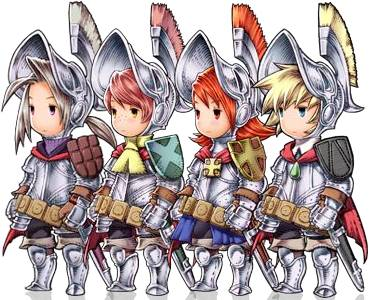
\includegraphics[width=\columnwidth]{./art/jobs/sentinel.jpg}\ofrow
	\accf{Sentinelas} são mestres do combate defensivo e raramente caem em combate. 
	Sua habilidade especial os permite não somente suportar grandes quantidades de danos, mas também proteger aliados. 
	Uma sentinela capaz é geralmente a última coisa entre o grupo e a morte certa.
}
{Espada}{Armadura Pesada}{
	Nível 1: & PV~+27 & PM~+16 & AGI~+3 & FOR~+1  \\
	Nível 2: & PV~+10 & PM~+10 & DEF~+1 & RES~+1 \\
	Nível 3: & \multicolumn{3}{l}{Bônus de Atributo do Arquétipo} \\
	Nível 4: & PV~+10 & PM~+5  &  DEF~+1 & FOR~+1 \\ 
	Nível 5: & PV~+10 & PM~+5  & RES~+1 & DEF~+1 \\ 
	Nível 6: & PV~+10 & PM~+10 & FOR +1 &        \\
	Nível 7: & PV~+10 & PM~+5  & DEF +2 &        \\
	Nível 8: & PV~+10 & PM~+5  & FOR +1 & DEF~+1 \\
	Nível 9: & PV~+10 & PM~+10 & FOR +1 &        \\
	Nível 10: & PV~+10  & PM~+10 & DEF +1 
}{
	\ofjobtech{Proteção}{3}{0r}{Único}{Você}{Ganhe AuDEF até o final de seu próximo turno.}{\enndef}{1}\ofabilitygap
	\ofjobtech{Primeiros Socorros}{6}{1r}{Único}{1u}{%
		Ao começar a usar essa habilidade, o alvo recupera PV igual ao seu nível atual. Se você não receber dano até o fim da conjuração e o alvo ainda estiver ao alcance, ele também recebe AuDEF e Acelerado por 1 rodada.}{}{2}\ofabilitygap
	\ofjobtech{Ameaçar}{6}{0r}{Único}{5u}{O alvo faz um teste de DF~8 ou fica Imóvel por 3 rodadas.}{\immobile}{4}\ofabilitygap
	\ofjobtech{Proteção Médica}{9}{0r}{Única}{Você}{Ganhe AuDEF e Regenerando por 3 rodadas.}{\enndef}{6}\ofabilitygap
	\ofjobtech{Formação Defensiva}{10}{0r}{2u}{Você}{Você e aliados dentro da área de efeito ficam Oscilando por 2 rodadas.}{\blink}{8}\ofabilitygap
	\ofjobtech{Proteção Poderosa}{26}{1r}{Único}{Você}{Pelas próximas 3 rodadas, ganhe Resistência contra danos físicos e mágicos.}{}{10}
}{
	\ofarchetypet{Defensor}
	{PV~+17 & PM~+3 & FOR~+2 & DEF~+1}
	{\ofarchetypetecha{Debilitar}{6}{0r}{Único}{1u}{Ao atacar com sucesso, o alvo também sofre ReFOR e ReMAG por 2 rodadas.}{\destr \demag}}
	{\ofarchetypepassive{Provocar}{Ao atacar com sucesso, é possível provocar o inimigo. Então, ele faz um teste de DF~8 ou o alvo dele tem que ser você, se possível, até o próximo turno dele.}}
	{\ofarchetypereaction{Bloqueio}{Sempre que um inimigo dentro de 2u de você tenta se afastar, ele faz um teste de DF~8. Se falhar, ele fica Imóvel até o começo do próximo turno dele.}}
	{\ofarchetypetechb{Retribuição}{14}{0r}{Único}{1u}{O alvo recebe dano igual à diferença entre seu PV atual e máximo.}{}}
}{
	\ofarchetypet{Paladino}
	{PV~+10 & PM~+15 & RES~+2}
	{\ofarchetypetecha{Muro de Terra}{8}{0r}{3u (Linha)}{8u}{Crie um largo muro de terra de 3u de altura que bloqueia o caminho. Ele se quebra depois de 3 rodadas ou ao sofrer um total de 20 de dano. Não pode usar essa habilidade se o muro anterior ainda estiver de pé.}{}}
	{\ofarchetypepassive{Proteção Sagrada}{Enquanto houver pelo menos 1 aliado a 1u de você, vocês ganham AuRES.}}
	{\ofarchetypereaction{Cobertura}{Sempre que um aliado dentro de 1u de você receber dano físico, você pode decidir direcionar pra si metade desse dano.}\nolinebreak}
	{\ofarchetypetechb{Astra}{10}{0r}{Único}{5u}{Pelas próximas rodadas, o alvo ganha AuRES e se torna Imune a todos os Efeitos de Estado.}{\enres}}
}
%
%
%
%
%
\ofjob{Invocador}
{
	\ofquote{"Não gosto do seu plano. É uma merda."\\}{Yuna}\ofrow
	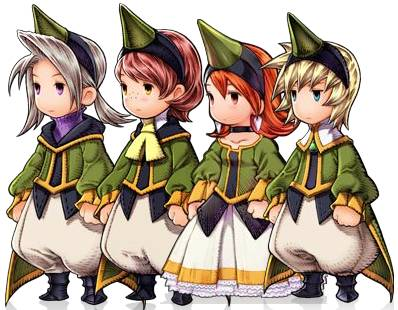
\includegraphics[width=\columnwidth]{./art/jobs/summoner.jpg}\ofrow
	Muitos heróis poderosos são capazes de invocar criaturas, mas o vínculo criado pelos \accf{Invocadores} são muito mais fortes, permitindo-os manifestar invocações por um longo período de tempo, para lutar ao seu lado no campo de batalha. 
}
{Cajado or Bastão}{Robe}{
	Nível 1: & PV~+16 & PM~+24 & AGI~+2 & FOR~+1 \\ 
	Nível 2: & PV~+5  & PM~+10 & RES~+1 & MAG~+1 \\ 
	Nível 3: & \multicolumn{3}{l}{Bônus de Atributo do Arquétipo}   \\
	Nível 4: & PV~+5  & PM~+10 & RES~+1 & DEF~+1 \\ 
	Nível 5: & PV~+5 & PM~+5  & RES~+2 & MAG~+1 \\  
	Nível 6: & PV~+10 & PM~+10 & DEF~+1 \\  
	Nível 7: & PV~+5 & PM~+10 & RES~+1 &  MAG~+1      \\  
	Nível 8: & PV~+5 & PM~+10 & DEF~+1 &		  \\  
	Nível 9: & PV~+10 & PM~+5  & MAG~+1 & RES~+1 \\  
	Nível 10: & PV~+10 & PM~+10 & FOR~+1 &        	  
}{
	\ofjobspell{Invocar}{8}{1r}{1u}{1u}{
		Manifeste uma criatura, você tem a habilidade de invocar, no campo de batalha.
		Em combate, invocações agem no turno após o seu e seguem os seus comandos. 
		Eles são dispensados ao sofrer KO, se você invocar novamente ou ao final da batalha.
		O PV \& PM da invocação é o mesmo de quando ele foi dispensado, se ele sofreu KO, ele é invocado com 1 de PV. 
		Eles recuperam totalmente seu PV \& PM ao dormir.
		A invocação sobe de nível com você e recebem os mesmos ganhos de atributo.
		As invocações e suas habilidades estão na próxima página.
	}{}{1}\ofabilitygap
	\ofjobpassive{Invocação: Carbuncle}{Ganhe a habilidade de invocar o \acc{Carbuncle}.}{1}\ofabilitygap
	\ofjobspell{Imagem}{6}{0r}{Único}{5u}{O alvo fica Oscilando por 3 rodadas.}{\blink}{2}\ofabilitygap
	\ofjobspell{Dissipar Magia}{10}{0r}{Único}{5u}{Todas as Resistências e Efeitos de Estado benéficos do alvo são removidos por 3 rodadas.}{}{6}\ofabilitygap
	\ofjobpassive{Invocar: Bahamut}{Ganhe a habilidade de invocar o \acc{Bahamut}.}{8}\ofabilitygap
	\ofjobspell{Invocação Final}{16}{1r}{1u}{1u}{
		Cause KO a uma criatura já invocada para invocar outra.
		A nova invocação recebe AuFOR, AuDEF, AuMAG, AuRES e Regenerando até o final da batalha.
	}{}{10}
}{
	\ofarchetypet{Devoto}
	{PV~+7 & PM~+13 & FOR~+1 & RES~+2}
	{\ofarchetypespella{Prece}{6}{0r}{1u}{Você}{Você e seus aliados na área de efeito recebem 2d de PV.}{}}
	{\ofarchetypepassive{Inferno}{Ganhe a habilidade de invocar o \acc{Ifrit} e Resistência permanente contra fogo. Além disso, sempre que um de suas invocações causam dano, adicione sua FOR e MAG ao total de dano causado por elas.}}
	{\ofarchetypereaction{Pacto de Sangue}{Sempre que sua invocação atual recebe dano, você pode redirecionar metade dele para você.}}
	{\ofarchetypespellb{Briza Curativa}{14}{0r}{5u (Linha)}{Você}{Você e seus aliados na área de efeito recuperam 4d de PV.}{}}
}{
	\ofarchetypet{Evocador}
	{PV~+12 & PM~+8 & MAG~+2 & DEF~+1}
	{\ofarchetypespella{Aero}{6}{0r}{Único}{4u}{Cause 2d de dano de Vento ao alvo.}{\wind} \ofabilitygap	\ofarchetypespella{Água}{6}{0r}{Single}{4u}{Cause 2d de dano de Água ao alvo.}{\water}}
	{\ofarchetypepassive{Rainha de Gelo}{Ganhe a habilidade de invocar a \acc{Shiva} e Resistência permanente a Gelo. Além disso, você pode usar magias e técnicas conhecidas pela sua invocação atual.}}
	{\ofarchetypereaction{Absorver Invocação}{Sempre que um das suas invocações sofrer KO em combate, recupere PV igual a seu nível atual x2, e também AuMAG por 3 rodadas.}}
	{\ofarchetypespellb{Aeroga}{14}{1r}{Único}{6u}{Cause 6d de dano de Vento ao alvo.}{\wind} \ofabilitygap \ofarchetypespellb{Águaga}{14}{1r}{Único}{6u}{Cause 6de da dano de Água ao alvo.}{\water}}
}
%
\clearpage
%
\ofmonster{Carbuncle}{1}{
\includegraphics[width=0.25\columnwidth]{./art/jobs/carbuncle.jpg}}
{
	PV: & \hfill 10 & PM: & \hfill 12\\
	FOR: & \hfill 1 & DEF: & \hfill 1 \\
	MAG: & \hfill 0 & RES: & \hfill 1 \\
	AGI: & \hfill 3 & Tamanho: & \hfill P\\
}
{\accf{Mordida}: 1d de dano(aumenta para 2d no Nível 5)}
{
	\mspell{Raio \hfill \accf{Nível 2}}{4}{0r}{Único}{3u}{Cause 2d de dano de Raio ao alvo.}{}
	\mspell{Refletir \hfill \accf{Nível 4}}{10}{0r}{Único}{3u}{O alvo ganha um escudo que reflete a próxima magia que o atingir de volta ao conjurador.}{}
	\mspell{Clarão \hfill \accf{Nível 7}}{8}{0r}{3u (Frontal)}{Você}{Todos os inimigos na área de efeito fazem um teste de DF~8 ou ficam Cegos por 3 rodadas.}{}
	\mspell{Muralha \hfill \accf{Nível 8}}{8}{0r}{Único}{5u}{O alvo ganha AuDEF e AuRES por 3 rodadas.}{}
	\mspell{Luz Rubi \hfill \accf{Nível 10}}{24}{1r}{2u}{8u}{Aliados na área de efeito ganham Regenerando por 3 rodadas e um escudo que reflete a próxima magia que os atingir de volta ao conjurador.}{}
}
%
\vspace*{1.8cm}\\
%
\ofmonster{Ifrit}{5}{
\includegraphics[width=0.28\columnwidth]{./art/jobs/ifrit.jpg}}
{
	PV: & \hfill 30 & PM: & \hfill 25\\
	FOR: & \hfill 3 & DEF: & \hfill 2 \\
	MAG: & \hfill 1 & RES: & \hfill 0 \\
	AGI: & \hfill 3 & Tamanho: & \hfill M\\
}
{
	\accf{Garras}: 2d de dano  (aumenta para 3d no Nível 8)\\
	\accf{Resistência}:\fire \hfill \accf{Fraqueza:}\ice
}
{	
	\mspell{Fogo \hfill \accf{Nível 5}}{4}{0r}{Único}{3u}{Cause 2d de dano de Fogo ao alvo.}{\fire}	
	\mtech{Golpe Flamejante \hfill \accf{Nível 5}}{5}{0r}{Você}{1u}{Ao atacar com sucesso, cause 2d de dano de Fogo adicional ao alvo.}{}	
	\mtech{Disparada \hfill \accf{Nível 7}}{8}{0r}{5u (Linha)}{Você}{Avance até 5u em linha à sua frente, causando 4d de dano a todos no caminho.}{}	
	\mspell{Fogaga \hfill \accf{Nível 8}}{12}{1r}{Único}{5u}{Cause 6d de dano de Fogo ao alvo.}{\fire}
	\mtech{Fogo Infernal \hfill \accf{Nível 10}}{20}{0r}{2u}{Você}{Inimigos na área de efeito sofrem 6d+10 de dano de Fogo.}{\fire}	
}
%
\newpage
%
\ofmonster{Bahamut}{9}{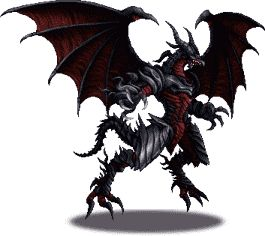
\includegraphics[width=0.3\columnwidth]{./art/jobs/bahamut.jpg}}
{
	PV: & \hfill 60 & PM: & \hfill 80\\
	FOR: & \hfill 5 & DEF: & \hfill 4 \\
	MAG: & \hfill 4 & RES: & \hfill 4 \\
	AGI: & \hfill 3 & Tamanho: & \hfill G\\
}
{
	\accf{Garras}: 3d de dano\\
	\accf{Imune}: Todo Efeito de Estado\hfill \accf{Resistência}:\dark\fire
}
{
	\mreaction{Ataque Final}{Se estiver prestes a cair a 0 PV, você pode usar uma de suas habilidades sem custo ou tempo de conjuração antes disso.}
	\mtech{Impulso \hfill \accf{Nível 9}}{12}{0r}{3u}{Você}{Inimigos na área de efeito sofrem 3d de dano de Escuridão.}{\dark}{}	
	\mtech{Baforada Destruidora \hfill \accf{Nível  9}}{14}{0r}{3u (Frontal)}{3u}{Todos na área de efeito fazem um teste de DF~8 ou sofrem 3d de dano e também ficam Envenenados e Cegos por 3 rodadas.}{\poison \blind}{}
	\mspell{Mega Labareda \hfill \accf{Nível 10}}{25}{2r}{2u}{10u}{Cause 6d+40 de dano, ignorando RES, a todos os inimigos na área.}{\fire}
}
%
\vfill
%
\ofmonster{Shiva}{5}{
\includegraphics[width=0.23\columnwidth]{./art/jobs/shiva.jpg}}
{
	PV: & \hfill 25 & PM: & \hfill 45\\
	FOR: & \hfill 2 & DEF: & \hfill 1 \\
	MAG: & \hfill 3 & RES: & \hfill 4 \\
	AGI: & \hfill 2 & Tamanho: & \hfill M\\
}
{
	\accf{Sincelo}: 2d de dano, 2u Alcance \hspace*{\fill} \accf{Fraqueza:}\fire\\
	(aumenta para 3d no Nível 8) \hspace*{\fill} \accf{Resistência}:\ice 
}
{	
	\mspell{Nevasca \hfill \accf{Nível 5}}{4}{0r}{Único}{3u}{Cause 2d de dano de Gelo ao alvo.}{}
	\mspell{Desproteger \hfill \accf{Nível 5}}{5}{0r}{Único}{5u}{O alvo recebe ReDEF por 3 rodadas.}{\dedef}
	\mspell{Descascar\hfill \accf{Nível 5}}{5}{0r}{Único}{5u}{O alvo recebe ReRES por 3 rodadas.}{\deres}
	\mspell{Muralha de Gelo \hfill \accf{Nível 7}}{12}{0r}{3u (Linha)}{5u}{Crie uma muralha de gelo de 3u de altura que bloqueia o caminho por 3 rodadas. Você não pode usar essa habilidade enquanto a parede anterior estiver de pé.}{}
	\mspell{Nevasga \hfill \accf{Nível 8}}{12}{1r}{Único}{5u}{Cause 6d de dano de Gelo ao alvo.}{\ice}
	\mspell{Pó de Diamante \hfill \accf{Nível 10}}{20}{0r}{3u (Frontal)}{Você}{Inimigos na área de efeito sofrem 6d de dano de Gelo e ficam Imóveis por 1 rodada.}{\ice\immobile}		
}
\clearpage
%
%
%
%
%
\ofjob{Ladrão}
{
	\ofquote{"Eu PREFIRO o termo "Caçador de Tesouros!""\\}{Locke}\ofrow
	
\includegraphics[width=\columnwidth]{./art/jobs/thief.jpg}\ofrow
	\accf{Ladrões} são lutadores ágeis, incomparáveis em "pegar emprestado"  itens de inimigos e têm um senso apurado para negócios que valem a pena.
}
{Adaga}{Armadura Leve}{
	Nível 1: & PV~+20 & PM~+19 & AGI~+4 \\
	Nível 2: & PV~+5  & PM~+10  & FOR~+1 & DEF~+1 \\
	Nível 3: & \multicolumn{3}{l}{Bônus de Atributo do Arquétipo} \\
	Nível 4: & PV~+10 & PM~+5  & FOR~+1 & DEF~+1 \\
	Nível 5: & PV~+10 & PM~+10 & FOR~+1 &        \\ 
	Nível 6: & PV~+5  & PM~+5  & DEF~+2 & RES~+1 \\ 
	Nível 7: & PV~+10 & PM~+10 & FOR~+1 &        \\ 
	Nível 8: & PV~+10 & PM~+5  & RES~+2 &        \\ 
	Nível 9: & PV~+5  & PM~+10 & FOR~+2 &        \\ 
	Nível 10:& PV~+10 & PM~+10  & DEF~+1 
}{
	\ofjobtech{Roubar}{3}{0r}{Único}{1u}{Faça um teste de DF~7 e tome algo do alvo. Role 1d e ganhe seu nível x20G em 1 ou 2, uma Poção em 3, um Remédio em 4, um Éter em 5 e uma Pena da Fênix em 6. O MJ pode determinar qualquer outro item.}{}{1} \ofabilitygap
	\ofjobtech{Escapar}{4}{0r}{3u}{Você}{Você e seus aliados na área podem se mover o dobro ao correr de seus inimigos por 3 rodadas.}{}{2} \ofabilitygap
	\ofjobtech{Dardo Envenenado}{7}{0r}{Único}{4u}{O alvo faz um teste de DF~8 ou sofre 1d de dano e um dos seguintes Efeitos de Estado à sua escolha por 3 rodadas: Envenenado, Imóvel ou Adormecido.}{}{4}\ofabilitygap
	\ofjobtech{Desaparecer}{8}{0r}{Único}{Você}{Torne-se invisível até 5 rodadas ou até agir. Enquanto isso, você está Oscilando e se acertar um ataque, sempre será um Acerto Crítico.}{\blink}{6} \ofabilitygap
	\ofjobtech{Dedos Pegajosos}{6}{0r}{Único}{Você}{Pelas próximas 3 rodadas, ao acertar um ataque, você também pode roubar o alvo sem custo adicional. Além disso, todos os itens pegos através de Roubar, são dobrados por essa duração.}{}{8} \ofabilitygap
	\ofjobtech{Réplica}{25}{1r}{Único}{1u}{Crie uma cópia exata de você que dura até 3 rodadas ou até criar outra. Ela age com você no seu turno, seguindo seu comando. A cópia pode usar as mesmas habilidade que você, exceto essa.}{}{10}
}{
	\ofarchetypet{Ninja}
	{PV~+14 & PM~+11 & FOR~+2}
	{\ofarchetypetecha{Arremessar}{4}{0r}{Único}{5u}{Lance um equipamento de seu inventário no alvo e cause dano a depender da categoria de equipamento dele. iniciante 1d, avançado 2d e especialista 3d. Você pode recolher todo item arremessado dessa maneira após a batalha.}{}}
	{\ofarchetypepassive{Ataque Antecipado}{Quando um aliado o escolhe para agir no próximo turno, aja imediatamente ao invés de esperar pelo turno do grupo adversário.}}
	{\ofarchetypereaction{Contra-ataque}{Quando um inimigo acerta uma ataque contra você, você pode atacá-lo, caso ainda esteja ao alcance.}}
	{\ofarchetypetechb{Assassinato}{14}{0r}{Único}{3u}{Mova-se para o próximo alvo e o ataque. Se acertar, ele faz um teste de DF~7 ou sofre KO.}{\ko}}
}{
	\ofarchetypet{Caçador de Tesouros}
	{PV~+10 & PM~+20 & DEF~+1 & RES~+1}
	{\ofarchetypetecha{Bolsos Rasos}{6}{0r}{Único}{Você}{Você pode usar um item logo após atacar.}{}}
	{\ofarchetypepassive{Gilionário}{Ao causar dano ao alvo, receba também uma quantidade de Gil igual ao dano total causado.}}
	{\ofarchetypereaction{Bater Carteira}{Ao se evadir de um ataque, você pode usar Roubar nele sem custo adicional.}}
	{\ofarchetypetechb{Jogar Gil}{5}{0r}{Único}{5u}{Lance uma quantidade de Gil até o máximo de 100G. O alvo sofre 1d de dano para cada 20G arremessados. O dinheiro é perdido no processo.}{}}
}
%
%
%
%
%
\ofjob{Engenhoqueiro}
{
	\ofquote{"Não dou a mínima se é ciência ou magia. Na verdade, eu acho que se tivesse que escolher, escolheria apostar na ciência."}{Cid}\\\\
	
\includegraphics[width=\columnwidth]{./art/jobs/tinker2.jpg}\ofrow
	\accf{Engenhoqueiros} são peritos técnicos que derrotam seus inimigos usando o poder da ciência. 
	Eles criam itens e dispositivos especiais que geram efeitos fantásticos em combate.
	Engenhoqueiros provam que qualquer tecnologia avançada é indistinguível de magia. 
}
{Arcos ou Arma ou Lança}{Robe}{
	Nível 1: & PV~+17 & PM~+24 & AGI~+2 & FOR~+1 \\
	Nível 2: & PV~+5  & PM~+10 & RES~+1 & DEF~+1 \\
	Nível 3: & \multicolumn{3}{l}{Bônus de Atributo do Arquétipo}  \\
	Nível 4: & PV~+5  & PM~+10 & FOR~+1 & DEF~+1 \\
	Nível 5: & PV~+10 & PM~+10  & FOR~+1 \\
	Nível 6: & PV~+10 & PM~+10 & RES~+1 \\
	Nível 7: & PV~+5  & PM~+10 & FOR~+1 & DEF~+1 \\
	Nível 8: & PV~+10 & PM~+10 & RES~+1 \\
	Nível 9: & PV~+10 & PM~+10 & RES~+1 \\
	Nível 10:& PV~+5  & PM~+10 & RES~+2
}{
	\ofjobtech{Estimulante}{4}{0r}{Único}{1u}{O alvo ganha Regeneração por 3 rodadas.}{\regen}{1}\ofabilitygap
	\ofjobtech{Lança Chamas}{4}{0r}{3u (Frontal)}{Você}{Ataque todos os inimigos na área. Se acertar, o dano causado é de Fogo.}{\fire}{2}\ofabilitygap
	\ofjobtech{Propelir}{6}{0r}{1u}{Você}{Você é impulsionado até 3u no ar de onde pode agir e se mover normalmente. Após 2 rodadas, você aterriza na sua posição atual.}{}{4}\ofabilitygap
	\ofjobtech{Posição Fortificante}{10}{0r}{2u}{5u}{Crie um Campo especial na área por 3 rodadas. Aliados ganham AuFOR e AuDEF enquanto estiverem dentro dela.}{\enstr\enndef}{6}\ofabilitygap	
	\ofjobtech{Onda de Choque}{9}{0r}{3u}{Você}{Todos na área, exceto você, recebem 3d de dano e são empurrados a 3u. Além disso, alvos afetados fazem um teste de DF~8 ou ficam Imóveis por 1 rodada.}{\immobile}{8}\ofabilitygap
	\ofjobtech{Caixa de Pandora}{26}{1r}{5u}{Você}{Inimigos na área sofrem 4d de dano. Além disso, alvos afetados rolam 1d e sofrem um Estado de Efeito por 3 rodadas, entre os seguintes: 1-Imóvel, 2-Lento, 3-Mudo, 4-Envenenado, 5-Cego ou 6-Adormecido.}{\immobile\slow\silence\poison\blind\sleep}{10}
}{
	\ofarchetypet{Químico}
	{PV~+8 & PM~+17 & RES~+2}
	{\ofarchetypetecha{Super Vacina}{6}{0r}{Único}{1u}{O alvo recupera 1d de PV e se torna Imune a Envenenado, Mudo, Cego e viroses tipo gripe, por 3 rodadas.}{}}
	{\ofarchetypepassive{Conhecimento de Item}{Você pode usar Itens a uma distância de 3u e afetar todos dentro 1u do alvo. Ambos os efeitos também se aplicam a Estimulante, Super Vacina e à técnica Misturar.}}
	{\ofarchetypereaction{Auto-Poção}{Ao sofrer dano, você pode usar um item de imediato, mas somente uma vez por turno.}}
	{\ofarchetypetechb{Misturar}{10}{0r}{Único}{3u}{Use 2 itens no alvo e role 1d. Alvos aliados recuperam 3d de PV em 1-2, ficam Oscilando em 3-4 ou Acelerados em 5-6. Alvos inimigos sofrem 3d de dano em 1-2, ficam Imóveis por 3 rodadas em 3-4 ou Lento por 3 rodadas em 5-6. }{\blink\haste\immobile\slow}}
}{
	\ofarchetypet{Maquinista}
	{PV~+10 & PM~+10 & FOR~+2 & DEF~+1}
	{\ofarchetypetecha{Torreta Automática}{8}{0r}{1u}{1u}{Crie uma torreta na área por 3 rodadas. No início de cada turno, cause dano igual ao seu nível atual em um inimigo dentro de 3u dela.}{}}
	{\ofarchetypepassive{Sintetizar}{Ganhe FOR+1, DEF+1 ou RES+1 adicional por cada Matéria que tenha equipado.}}
	{\ofarchetypereaction{Defesa Balística}{Ao sofrer dano de um inimigo que está além de 2u de você, faça um teste de DF~7. Em caso de sucesso, o dano é reduzido pela metade.}}
	{\ofarchetypetechb{Raio de Satélite}{12}{0r}{?}{?}{Inimigos afetados sofrem 5d de dano. Escolha uma das seguintes formas para determinar os alvos afetados: desenhe um largo círculo de 1u ao seu redor com um raio de até 8u \accf{ou} desenhe uma linha larga de 1u ao seu redor com ambas extremidades a 8u de você \accf{ou} todos os inimigos dentro de 5u de você fazem um teste e todos que obterem um número ímpar são afetados. }{}}
}
%
%
%
%
%
\ofjob{Mago do Tempo}
{
	\ofquote{"Tempo... Não esperará."\\}{Ultimecia}\\\\
	
\includegraphics[width=\columnwidth]{./art/jobs/timemage.jpg}\ofrow
	\accf{Magos do Tempo} são mestres do tempo e espaço e entendem que imaginação é mais importante do que conhecimento. 
	Eles manipulam o fluxo do tempo e dobram o tecido da realidade em seu benefício.
}
{Cajado}{Robe}{
	Nível 1: & PV~+17 & PM~+27 & AGI~+2 & MAG~+1 \\
	Nível 2: & PV~+5  & PM~+10 & RES~+1 & FOR~+1 \\
	Nível 3: & \multicolumn{3}{l}{Bônus de Atributo do Arquétipo}  \\
	Nível 4: & PV~+10  & PM~+10 & MAG~+1 &        \\ 
	Nível 5: & PV~+10 & PM~+10 & RES~+1 &		  \\ 
	Nível 6: & PV~+5  & PM~+10 & DEF~+1 & RES~+1 \\ 
	Nível 7: & PV~+5  & PM~+10 & RES~+2 \\ 
	Nível 8: & PV~+10  & PM~+10 & DEF~+1 \\ 
	Nível 9: & PV~+5  & PM~+10 & RES~+2 &        \\ 
	Nível 10:& PV~+5  & PM~+10 & MAG~+1 &	RES~+1	  
}{
	\ofjobspell{Gravidade}{6}{0r}{Único}{3u}{O alvo sofre 2d de dano e só  se move metade do normal no próximo turno dele.}{}{1}\ofabilitygap
	\ofjobspell{Acelerar}{8}{0r}{Único}{5u}{O alvo fica Acelerado por 3 rodadas.}{\haste}{2}\ofabilitygap
	\ofjobspell{Retardar}{8}{0r}{Único}{5u}{O alvo fica Lento por 3 rodadas.}{\slow}{2}\ofabilitygap
	\ofjobspell{Flutuar}{8}{0r}{Único}{3u}{O alvo levita até 3u acima do chão por 3 rodadas. Enquanto aliados ainda podem se mover enquanto no ar, inimigos ficam Imóveis.}{}{4}\ofabilitygap
	\ofjobspell{Gravidaga}{15}{1r}{2u}{6u}{Inimigos na área sofrem 6d de dano e um Campo Vagaroso surge, durando 3 rodadas.}{}{6}\ofabilitygap
	\ofjobspell{Interromper}{16}{0r}{30u}{Você}{Inimigos na área fazem um teste de DF~8 ou ficam Adormecidos por 1 rodada.}{\sleep}{8}\ofabilitygap
	\ofjobspell{Banimento}{26}{0r}{Único}{5u}{Bana temporariamente o alvo para outra dimensão. Se for um aliado, ele ainda pode agir, mas não interagir com o campo de batalha. Após 3 rodadas, o alvo reaparece no mesmo lugar, qualquer um naquele lugar é empurrado e sofre 6d de dano. Você não pode Banir o mesmo alvo consecutivamente ou se o efeito anterior ainda continuar.}{}{10}
}{
	\ofarchetypet{Ilusionista}
	{PV~+5 & PM~+20 & MAG~+2}
	{\ofarchetypespella{Teleporte}{6}{0r}{1u}{5u}{Teleporte-se para um espaço desocupado de sua escolha e que possa ver, até 5u.}{}}
	{\ofarchetypepassive{Tunelamento}{Ao conjurar uma magia, você pode escolher dobrar seu alcance e distancia de alvo, mas o custo em PM também é dobrado.}}
	{\ofarchetypereaction{Teleporte Rápido}{Ao ser alvo de um ataque, você pode tentar teleportar. Neste caso, faça um teste de evadir-se com vantagem e, se bem sucedido, a teleportação se torna adicional à evasão, ou seja, sem custo em PM.}}
	{\ofarchetypespellb{Troca}{14}{0r}{Único}{10u}{Escolha dois alvos dentro do alcance e troque suas posições. Inimigos sofrem 4d de dano adicional, enquanto aliados causam 4d de dano a todos a 2u de suas novas posições. Além disso, ambos alvos afastam qualquer coisa que impediria suas novas posições.}{}}
}{
	\ofarchetypet{Oráculo}
	{PV~+8 & PM~+17 & FOR~+1 & RES~+1}
	{\ofarchetypespella{Estender}{5}{0r}{Único}{8u}{A duração de todos os Efeitos de Estados ou benefícios recebidos no alvo, duram mais 3 rodadas.}{}}
	{\ofarchetypepassive{Antecipar-se}{Antes do começo de cada combate, ganhe um turno extra, mesmo se o inimigo tiver rodada surpresa. }}
	{\ofarchetypereaction{Destino}{Quando um magia ou técnica mirar alguém dentro de 5u e acertar, você pode atrasá-la. Neste caso, a habilidade só funciona de fato 1 rodada depois. Esse efeito não acumula.}}
	{\ofarchetypespellb{Ímpeto}{12}{0r}{Único}{5u}{O alvo tem um turno extra antes de terminar o seu próprio, mas só uma vez por rodada. Após isso, você ainda pode escolher o próximo a agir do lado do seu grupo normalmente. }{}}
}
%
%
%
%
%
\ofjob{Guerreiro}
{
	\ofquote{"Sonhei que era um imbecil."\\}{Squall}\\\\
	
\includegraphics[width=\columnwidth]{./art/jobs/warrior.jpg}\ofrow
	\accf{Guerreiros} são especialisas em combate corporal e possuem um um ataque e defesa fortes. 
	São proficientes em poderosas espadas e armaduras, tornando-os mais perigosos e duráveis.
}
{Espada}{Armadura Leve e Pesada}{
	Nível 1: & PV~+25 & PM~+18 & AGI~+3 & FOR~+1 \\
	Nível 2: & PV~+10 & PM~+5  & FOR~+1 & DEF~+1 \\
	Nível 3: & \multicolumn{3}{l}{Bônus de Atributo do Arquétipo}  \\
	Nível 4: & PV~+10 & PM~+5  & FOR~+2 &        \\ 
	Nível 5: & PV~+10  & PM~+10 & DEF~+1 \\ 
	Nível 6: & PV~+10 & PM~+5  & DEF~+1 & RES~+1 \\ 
	Nível 7: & PV~+10 & PM~+10  & FOR~+1 &        \\ 
	Nível 8: & PV~+10 & PM~+5  & RES~+2 &        \\ 
	Nível 9: & PV~+5  & PM~+10 & FOR~+1 & DEF~+1 \\ 
	Nível 10:& PV~+10 & PM~+5  & DEF~+2 &         
}{
	\ofjobtech{Avançar}{3}{0r}{Único}{1u}{Se acertar o ataque contra o alvo, empurre-o para trás 1u além do dano causado.}{}{1}\ofabilitygap
	\ofjobtech{Surrar}{6}{0r}{Único}{1u}{Ao atacar um alvo que tenha vantagem no teste de evasão e acertar, será um Acerto Crítico.}{}{2}\ofabilitygap
	\ofjobtech{Vitalidade}{5}{0r}{Único}{Você}{Pelas próximas 3 rodadas, efeitos de restaurar seu PV ou PM são dobrados. Além disso, ao fazer um teste para resistir a um efeito, a DF tem -2.}{}{4}\ofabilitygap
	\ofjobtech{Exército de um Homem Só}{10}{0r}{3u}{Você}{Ataque cada inimigo na área rolando um dano que se aplica a todos que falharem em se evadir. Após isso, você pode se mover para próximo de qualquer um dos alvos afetados.}{}{6}\ofabilitygap
	\ofjobtech{Coragem}{10}{0r}{2u}{Você}{Você e seus aliados dentro da área de efeito ganham AuFOR e AuMAG por 2 rodadas.}{\enstr \enmag}{8}\ofabilitygap
	\ofjobtech{Múltiplos Golpes}{28}{0r}{Único}{1u}{Faça 3 ataques contra o alvo. Sempre que ele rolar 4 ou menos no teste de evasão, você consegue um Acerto Crítico.}{}{10}
}{
	\ofarchetypet{Cavaleiro Negro}
	{PV~+5 & PM~+15 & DEF~+1 & RES~+2}
	{\ofarchetypetecha{Quebrar Defesa}{6}{0r}{Single}{1u}{Ao acertar um ataque, o alvo também sofre ReDEF e ReRES por 2 rodadas.}{\dedef \deres}}
	{\ofarchetypepassive{Devorador de Alma}{Ao acertar um ataque, também cause dano de Escuridão igual à metade do dano causado, a si mesmo e a todos os inimigos a ~3u de você.}}
	{\ofarchetypereaction{Preço em Sangue}{Sempre que um inimigo gastar PM, você pode forçá-lo a gastar o mesmo em PV, se tiver o suficiente. Após isso, recupere PV igual ao valor perdido dessa forma, pelo alvo.}}
	{\ofarchetypetechb{Enfurecido}{10}{0r}{Único}{5u}{Pelas próximas 3 rodadas o alvo só pode atacar, mas cada acerto é um Acerto Crítico. Se mirar um inimigo, ele faz um teste de DF~8 ou é afetado.}{}}
}{
	\ofarchetypet{Samurai}
	{PV~+16 & PM~+9 & FOR~+2}
	{\ofarchetypetecha{Foco}{5}{0r}{Alvo}{Você}{Pelas próximas 3 rodadas, o inimigo atacado terá desvantagem em testes de evasão.}{}}
	{\ofarchetypepassive{Mutilar}{Sempre que o alvo de seus ataques rolar 5 ou menos no teste de evasão, ele recebe um dos seguintes Efeitos de Estado: Imóvel, Cego ou ReFOR.}}
	{\ofarchetypereaction{Bushido}{Você pode se evadir de Técnicas ao passar no teste de evasão. Além disso, se for bem sucedido, recupere PM igual ao seu nível atual.}}
	{\ofarchetypetechb{Tempestade de Lâmina}{8}{0r}{5u (Linha)}{Você}{Todos na área sofrem 4d de dano.}{\wind}}
}
%
%
%
%
%
\ofjob{Mago Branco}
{
	\ofquote{"Ei, essa frase é do Cloud! 'É muito perigoso, não posso me envolver...' blá, blá, blá."\\}{Aerith}\\\\
	
\includegraphics[width=\columnwidth]{./art/jobs/whitemage.jpg}\ofrow
	\accf{Magos Brancos} são peritos em magias defensivas, de recuperação e proteção. 
	São medíocres em combate físico, mas possuem alta resistência contra magias.
}
{Cajado}{Robe}{
	Nível 1: & PV~+19 & PM~+25 & AGI~+2 & FOR~+1 \\
	Nível 2: & PV~+5  & PM~+10 & MAG~+1 & RES~+1 \\
	Nível 3: & \multicolumn{3}{l}{Bônus de Atributo do Arquétipo} \\
	Nível 4: & PV~+10 & PM~+5 & MAG~+1 & DEF~+1	  \\
	Nível 5: & PV~+5  & PM~+10 & RES~+1 &	FOR~+1  \\ 
	Nível 6: & PV~+5  & PM~+5 & MAG~+2 &        \\ 
	Nível 7: & PV~+10  & PM~+10 & RES~+1 & DEF~+1 \\ 
	Nível 8: & PV~+5 & PM~+5  & MAG~+2 & DEF~+1 \\ 
	Nível 9: & PV~+5  & PM~+10 & RES~+1 &	MAG~+1   \\ 
	Nível 10:& PV~+10 & PM~+10 & RES~+1 &	        
}{	
	\ofjobspell{Cura}{4}{0r}{Único}{3u}{O alvo recupera 2d PV.}{}{1}\ofabilitygap
	\ofjobspell{Drenar}{6}{0r}{Único}{3u}{Cause 1d de dano ao alvo e recupere PV na mesma quantidade.}{}{2}\ofabilitygap
	\ofjobspell{Esuna}{6}{0r}{Único}{5u}{Remova todos o Efeitos de Estado negativos, exceto KO, do alvo.}{}{4}\ofabilitygap
	\ofjobspell{Curaga}{14}{1r}{2u}{5u}{Alvos na área recuperam 6d PV.}{}{6}\ofabilitygap
	\ofjobspell{Dispersar}{6}{0r}{5u}{50u}{Remova um Campo de Efeito dentro da área.}{}{6}\ofabilitygap
	\ofjobspell{Sagrado}{21}{2r}{Único}{12u}{Cause 6d+45 de dano Sagrado ao alvo.}{\holy}{8}\ofabilitygap
	\ofjobspell{Auto-Ressurreição}{28}{2r}{Único}{3u}{Invoque um anjo guardião que  zela por você. Na próxima vez que você ficar KO, seja revivido com 1 PV. Esse efeito não acumula e se não ativado, expira se o alvo dormir. }{\ko}{10}
}{
	\ofarchetypet{Sábio}
	{PV~+11 & PM~+9 & MAG~+2 & FOR~+1}
	{\ofarchetypespella{Adormecer}{6}{0r}{Único}{5u}{O alvo faz um teste de DF~8 ou fica Adormecido por 3 rodadas.}{\sleep}
		\vspace*{0.1cm}\\ \ofarchetypespella{Silenciar}{6}{0r}{Único}{5u}{O alvo faz um teste de DF~8 ou fica Mudo por 3 rodadas.}{\silence}}
	{\ofarchetypepassive{Sabedoria Anciã}{Ao causar um ou mais Efeitos de Estado ao alvo, você também pode causar ReDEF ou ReRES a ele por 3 rodadas.}}
	{\ofarchetypereaction{Absorver PM}{Ao ser alvo de uma habilidade, recupere seu PM igual ao PM gasto pelo conjurador.}}
	{\ofarchetypespellb{Maldição}{14}{1r}{Único}{5u}{O alvo faz um teste de DF~9 ou sofre 4d de dano e fica Envenenado e Zumbi por 3 rodadas.}{}}
}{
	\ofarchetypet{Médico}
	{PV~+7 & PM~+13 & RES~+2 & DEF~+1}
	{\ofarchetypespella{Proteger}{4}{0r}{Único}{5u}{O alvo ganha AuDEF por 3 rodadas.}{\enndef} \vspace*{0.1cm}\\ \ofarchetypespella{Concha}{4}{0r}{Único}{5u}{O alvo ganha AuRES por 3 rodadas.}{\enres}}
	{\ofarchetypepassive{Ética Médica}{Ao usar Magia em um aliado até 1u, você também pode usar um item de imediato.}}
	{\ofarchetypereaction{Sem Efeito Colateral}{Sempre quando seria afetado por uma magia ou técnica não sendo o alvo primário dela, você pode escolher que você e todos os alvos secundários não serão afetados.}}
	{\ofarchetypespellb{Ressuscitar}{22}{2r}{Único}{5u}{Remova KO do alvo  e ele fica com PV cheio.}{\ko}}
}
